\section{Results and Discussion}

General discussion..

\subsection{Classifiers}

\textbf{Transfer Learning using ImageNet.} Classifiers trained on imagenet are tuned towards natural images. While VGG19 and Xception perform better than the shallower LeNet, their full performance only develops when training from scratch. This shows how natural images are truely different than infographics.
\\~\\
\textbf{Anti-aliasing.} Does it help? Not sure yet!




%
%\subsection{Elementary Perceptual Tasks}
%
%
%\subsection{Position-Angle Experiment}
%
%
%\subsection{Position-Length Experiment}
%
%\subsection{Bars and Framed Rectangles Experiment}
%


%\begin{figure}[t]
%	  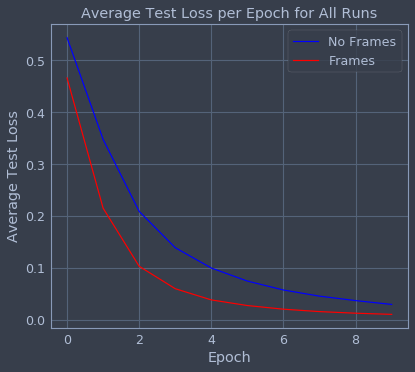
\includegraphics[width=\linewidth]{figure12_val_loss.png}
%  \caption{\textbf{Classifier Efficiency of the Bars and Framed Rectangles experiment.} Categorical Cross-Entropy loss for the \emph{bars and framed rectangles experiment} as described by Cleveland and McGill~\cite{cleveland_mcgill}. The frame around the bars adds an additional visual cue enables faster network convergence. This is not yet reproducible!}
%	\label{fig:figure12_val_loss}
%\end{figure}
